\chapter{Dynamic digitalization of society}

\section{Scenarios of individuals}

From an epidemic perspective, the more agitated society is, the more an epidemic spreads. It is therefore necessary to describe the individual dynamics of each individual. The question of time is essential to deal with. Considering the diversity of trips on the same day and the use of SumoMobility, it is obvious to deal with dynamic digitalization day by day, on a minute scale. In practice, a second scale will be applied to adapt to the SumoMobility format.\\

How do I represent a 24-hour scenario ?\\

The idea is to present a sequence of spaces with defined slots as well as additional information specifying the movement such as a degree of importance or the role of the individual. All scenarios start at a fixed time in the day. As a rule, more active individuals are observed at 01:00, during the night, than at 05:00 in the morning. It therefore seems wise to specify a fixed start time of the scenarios at 04:00. The scenarios therefore begin with the awakening of the individual and end with his sleep. Of course, in theory, a scenario begins and ends at the same time. The greatest complexity of dynamic digitalization is the generalization of the creation of scenarios for each individual, respecting the diversity of situations. We can resume the parallel with a neural network.\\

\subsection{Multiple hyperparameters}

A scenario must consider several factors to meet this specific complexity :\\

\begin{itemize}

\item Infectious state of the individual : known states, actual states.\\
The infectious state primarily impacts an individual's scenario. The more severe its actual infectious state, the less attention is paid to the condition identified to it. On the other hand, the healthier its real state, the more interested one is in its known state. We can speak more of the propensity of the individual for a less serious condition and constraints/obligations for the individual with a serious condition. For more details, the infectious reflexes associated with each case are lower in the report.\\

\item Territorial decision :\\
Territorial decisions impose constraints on the population. These are the combinatorial solutions on which the reinforcement learning algorithm relies. This is the very basis of this search for multi-criteria optimization of the society. These territorial decisions are to be defined manually by describing the actions they apply to the digitalization. It should be noted that decisions may be associated with constraints/obligations on tests and vaccinations. For more details, the decisions are further discussed in a later section.\\

\item Type of day : weekday, saturday, sunday, holidays, seasonal period.\\
A person's daily life depends a lot on the calendar. Depending on the type of day, the scenario can be modeled quite differently. On weekdays, most people work during the day, have little free time in the late afternoon and then go out or stay at home in the evening. Otherwise, on weekends, they have most of their time to do what they want. The type of day is therefore an interesting parameter because it makes it easy to have information on the state of the dynamics in general. In addition, it is obvious that the time of year is a very important parameter to best characterize dynamic propensities. Individuals orient themselves more in parks in summer than in winter. In a later version, we can have fun with this calendar to have more tools and leverage to design realistic scenarios.\\

\item Type of daily life : work, rest, holidays\\
Each individual can have different daily scenarios regardless of the type of day. He can either have a work day where he spends a certain number of hours, defining, at work, or be at complete rest, or even go on vacation and get out of his routine completely.\\

\item Role of places : economical, necessary, unnecessary work\\
The role of places is important to clarify. From an economic evaluation point of view, it is essential to distinguish between the individuals who work or visit the different places. After that, it is also necessary to distinguish between necessary and unnecessary travel. This has little impact in a normal situation, but these specifications are more than necessary in case of restriction. For example, supermarkets, medical places and pharmacies are necessary travel. In a later version, it might be interesting to no longer represent the importance of places in binary terms but with a scale of necessity. For example, we could consider that gyms are a psychological ``outlet'' for individuals. These places could then be considered as semi-necessary locations. We return to an evolutionary perspective where we consider the habits of individuals, when these seem to be an individual need. Conversely, a center of attraction will always be denoted as unnecessary for example. Apart from the working role of places, this level of importance can be classified directly into place categories. This could also add a new psychological dimension to the project, which will be exposed at the end of the report. It should be noted that this has nothing to do with the ability of places to contaminate its occupants.\\

\item Various propensities : external travels, other accommodations, family or friendly visits, etc.\\
Each individual has a propensity to move outside the study area. Individuals residing near a boundary of the study area will be more likely to travel outdoors. We find the problem of identifying the proximity of places to the geographical limits of the region. Then, the individual may occasionally sleep elsewhere than at home, whether in the study area or not. We can also consider the propensity of the individual to share moments with friends and family. We find the perspective of evolution of the project where we specify the friends and family of each individual. It is in a way the hyperparameters for all the possible evolutions of dynamic digitalization, which will be useful among others to approach the observed affluences.\\

\item Type of space selection : assigned to the individual, random, criteria\\
When developing a scenario, you need to know what place to add to the sequence. So the question does not arise as to the base of the individual where housing and work are well identified. We join the representation of the habits of individuals, which can be associated with certain propensities. As for the rest, the daily life of an individual can be very diverse, and it is necessary to be able to choose places from the entire database. From a simplistic point of view, we can say that the individual visits a sequence of place a little randomly. In a certain set of categories, a location can be chosen completely randomly or according to certain criteria. The more random the selection of places, the more the circulation of the epidemic will have a significant Brownian motion. It may therefore be wise to perfect this selection by criteria such as the nearest or largest place within a certain radius of distance for example. It is therefore necessary to add filtration functions to select a place from the database. This hyperparameter could be perfected with voluntary population data on their preference, such as surveys.\\

\end{itemize}

\subsection{How do you do it ?}

Optimizing agendas for a population is already a complex problem. The idea here is to simplify this generalization of scenario with the parameters mentioned above. In order of importance, the scenarios depend first on the infectious state of the individual and then on territorial decisions, especially during major constraints/obligations. Then, we can identify travel patterns according to the type of day and the type of daily life of the individual. Then we have the various propensities of the individual to organize certain necessary or non-necessary trips. For the rest, it is a question of identifying the places to be introduced into the sequence, whether it is already predefined, chosen according to certain criteria, categories or entirely random, etc.\\

Each individual has certain necessities that he must realize according to a certain rhythm over time. This is the case, for example, with food shopping or routine medical visits. It is not realistic to reproduce this kind of travel every day. It is therefore necessary to establish a system of propensity of the individual to build his daily life. A first approach could be to reproduce more or less the same system as a shared distribution of computer tasks on the same computing core, where the tasks would represent all available travel. Each available move has a score that increments over each day. It will be necessary to separate them by necessity or not. By considering the score of each of them, the individual would select the most appropriate one in his daily life.\\

The selection lever could be a threshold system from which the individual would place the displacement in his scenario. It would then be necessary to respect the space available and the competition of trips exceeding this threshold. It would seem wise to choose an identical threshold for all places and to change the daily increase in the propensity score of each category. Another leverage system could be to integrate these movements while playing with stochastic processes. These stochastic decisions would be made every day, regardless of the time. An identical increment would then be applied for all categories of places. Differentiation would be added by factors specific to each of these categories. Regardless of the selection lever, the scores of each category would be reset to zero each time they are selected.\\

\subsection{Problem of time}

Time is the major constraint when designing a scenario. A scenario must not exceed 24 hours. There are two options for taking into account the time limit. A bit like the backpack problem, a scenario has a time limit and it must be filled with trips that have a certain importance/obligations, while not exceeding this limit. Then either the scenario can be built iteratively. Either we first select all the trips of the day and then we arrange them with timings. In theory, we should reproduce the conception of a scenario in our daily lives : we must all respect time slots and adapt to the time we have left.\\

There is a certain complexity to take into account : we can not predict the travel time of the individual, hence the interest of using \textit{SumoMobility} to have the temporal aspect of the trips. We will see later that the project cadence the scenarios by the departures of individuals in the direction of each places, which therefore includes the unpredictable travel time as well as the time within each places. It is necessary to have estimations for each of its trips, considering the type of transport and the desired duration on site. What interests us in this project is the actual time of each individual in the places.\\

There is a significant problem in poorly timing travel. If a time between two timings is too short, the individual may not have time to complete his journey towards a place that he will already have to start the next trip towards the next location. In practice, there would be no problem when running with \textit{SumoMobility}. But once the simulation is done, the analysis phase will not be able to properly evaluate the scenarios knowing that some places will not actually be visited.\\

It might be interesting to specify a reference on the occupancy times of individuals in places. Each category of place could therefore be characterized by a typical duration of passages, whether for a simple visit, a working time, etc. This duration could be represented by a fixed quantity or a positive normal distribution, parametrized by a certain mean and a certain standard deviation. Note that we can already find a random duration in practice since we do not anticipate the exact travel time. An interesting estimation of this travel time could be made depending on the type of transport and the distance between the point of departure and the point of arrival. For example, a linear regression between distance, type of transport and the actual travel time can be performed.\\

Timings must also follow a certain coherence to group individuals in their dynamics. For example, individuals have fairly general slots for meal times. Work timings depend on the type of work of the individual, etc.\\

\subsection{Memory management}

The question of memory management of each individual's scenarios is an interesting point. The basic problem is whether a scenario is unique over time ? For the sake of ease, we may prefer a memory management of scenarios.\\

To simplify, we can initialize several scenarios for each individual according to certain conditions, even if it means editing them according to their infectious state or political decisions, for example. This design would therefore be interesting to take into account the individuality of each individual and the calendar. For each day of simulation, this means removing the construction time from each scenario and replacing it with a time to adapt to the conditions.\\

However, we have previously noted that the most impactful parameters when constructing scenarios are political decisions and infectious reflexes. From an execution point of view, this would increase the memory requirement of the program but accelerate the time of digitization. However, we would lose some diversity and an unpredictable side of mobility.\\

The other conception would be not to keep in memory the scenarios but to build them every day of digitization. Compared to the first option, it would then be necessary to keep the tools for constructing scenarios for each individual such as propensity scores, etc.\\

\newpage

\section{SumoMobility}

\textit{SumoMobility} is an application simulating urban traffic from map data of a road network. By taking an \textit{openstreetmap} file and applying pre-processing, we can circulate individuals through the different real places. It is possible to use public transport in the area described by the \textit{openstreetmap} file with the actual positions of the stops. As a reminder, each individual is initialized with a means of transport, according to his age and certain proportions. For the efficiency of the project, it will be limited to a simplistic use of travel. The interest is to consider only the travel times of individuals in daily traffic, and to have an overview of the infectious risks in public transport.\\

Indeed, public transport is also a place to be taken into account in the spread of infectious agents, although it is not listed in the place database. This consideration can be done globally for simplicity : we can look at the ratio between the proportion of infectious and non-infectious people using public transport as well as the frequency of this public transport. An overall assessment score can thus be provided to the infectious assessment function of the individual ; this score will only be taken into account if the individual takes public transport. Of course, this consideration can be further refined to make it more individualistic.\\

\begin{figure}[h]
  \centering
  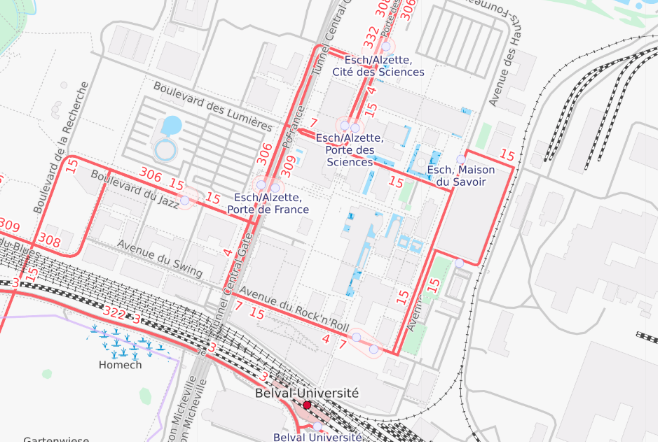
\includegraphics[width=0.8\linewidth]{media/belval_osm_tp.png}
  \caption{\centering {\small An overview of public transport data in the openstreetmap format.}}
  \label{fig:belvalosmtp}
\end{figure}

To simplify the use of \textit{SumoMobility}, the simulation of a day in society is carried out without making pedestrians interact with each other. This avoids unnecessary calculations in our use, and also avoids unpredictable bugs. For example, one of these irregularities can be the collision/traffic jam of several individuals on a pedestrian lane, which causes serious problems on digitalization. Such considerations in the field of epidemic spreading are unnecessary and even very problematic for the project. Similarly, in a simplistic case, we are not interested in \textit{SumoMobility}'s advanced options such as recalculating trips according to traffic, managing low beams or using taxis. In our simple use, however, some parameters are to be adjusted :\\

\begin{itemize}

\item We must manually choose the frequency of passage of vehicles in the automatic generation of public transport with the stops and lines described by the \textit{openstreetmap} file. This is an important parameter for individuals who travel by public transport, whether for the speed or the risk of contamination of their travel. However, it is quite easy to find information on the average frequency of public transport in a region, or simply to enter a frequency that seems realistic. It would be interesting to separate the different classes of public transport in a later version in order to apply different frequencies of passage to them.\\

\item It is interesting to look at the parking constraint of vehicles. In a simplistic version, it is assumed that individuals travelling by car do not need to leave their vehicle in a parking lot ; cars appear and disappear directly at the pedestrian crossing. This parameter is not that important in the  digitalization of an epidemic. Of course, in the practical case, this could represent the time that dwellers spend to find parking in the city, including the time and the flat-rate constraints of car parks. Conversely, this option would be very interesting with a view to perfecting dynamic digitalization or civil engineering.\\

\end{itemize}

The simulation is continuous over time and travel under \textit{SumoMobility} is done only by considering the road network. Therefore, to model the stop of an individual in a place, it is necessary to route the individual to the road that is closest to this place. For simplicity, the trips between the different places are made with the same type of transport, unique and assigned to each individual.\\

To make the connection between individuals' scenarios and their implementation as trips in \textit{SumoMobility}, it is necessary to make some changes. From the scenarios of individuals, it is necessary to be able to write the trips of the individuals which will then be translated into routes by a specific algorithm of \textit{SumoMobility}, called \textit{duarouter}. This router is very technical and has many options to identify the fastest sequence of routes to connect a starting and an arrival route. It is possible to adjust many parameters related to optimization such as the vehicles that can be driven on each road, the speed limits on each road, the detailed speeds of each vehicle, etc. The algorithm he uses is Dijkstra. For simplicity, we do not worry about this optimization since it is not the subject of this project. This tool simply allows us to find sensible movements between points of interest. However, we are concerned about the connectivity of the road network, which we can try to correct directly with the router, so as not to have an error in the path search. In this acquisition, the algorithm can use public transport, for individuals using the public transport mode, which will have already been introduced and timed previously. An undeniable advantage of \textit{duarouter} is the ability to perform calculations on several threads and speed up this process. In particular, this is not negligible when the scenarios of individuals evolve over the days and the routing step must be done regularly. \\

The router automatically creates vehicles with a unique identifier per individual. Each vehicle then makes the trip corresponding to a trip. The total itinerary of the individual therefore designates the unique identifiers of these vehicles to carry out the trips associated with these vehicles. However, this design presents a problem when the individual owns a car and passes through many places : the stops of the individual, representing the stop in each places during the scenario, cannot be introduced between the same chain of trips. The individual cannot therefore use his car to make two different trips. The trip of his car corresponds to the first movement of the individual, i.e. the first sequence of trips, without stops, of the individual.\\

One of the ways for correction would be to model the trip of the individual's single car, including the individual's stops. However, this does not seem to be feasible since \textit{duarouter}. It is from this problem that we must separate the total daily itinerary of the individual in simple trips. However, since we cannot predict the travel time of the first trip, we must estimate the timings on all subsequent trips. In an ideal case, it would certainly have been more interesting to consider only the occupancy time of individuals in places, without worrying about estimates of transport times.\\

With this design, the scenario of each individual is divided into several subpaths, identified by the identifier of the person to which are added specific characters that increment with the number of trips. The same individual, under different trip identifiers, can use several cars for different trips. A trip thus becomes the simple passage from one place to another. As a reminder, we do not take into account the duration that the individual occupies a place but the timings where the individual wishes to move into a place. The duration of the individual's occupation in a location is then reanalyzed after \textit{SumoMobility} is executed. The decomposition of an individual's scenario into several trips is done contiguously in the routes file, which removes the chronological order of all trips from the file. It is therefore necessary to apply an algorithm specific to \textit{SumoMobility} to reclassify in order all the routes in the file according only to the departure time of each trip.\\

\begin{figure}[h]
  \centering
  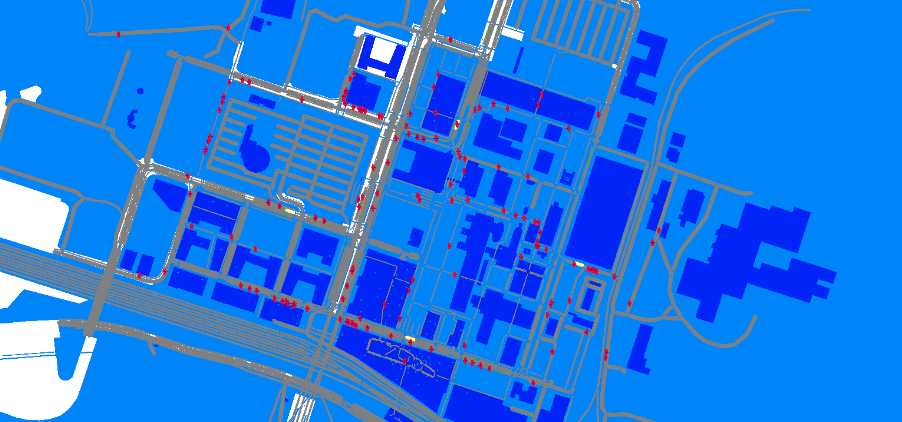
\includegraphics[width=\linewidth]{media/sumo_mobility.png}
  \caption{\centering {\small En example of graphical execution of SumoMobility here in the network of the Belval campus in Esch-sur-Alzette.}}
  \label{fig:sumomobility}
\end{figure}

In a first version of the graphical display, it is possible to observe the circulation of individuals in an environment described as in the example above. Regardless of their infectious status, individuals are described by red dots. The shapes in yellow correspond to vehicles such as cars or buses. The places that individuals travel through on a daily basis are depicted in dark blue. Of course, it could be interesting to review this display to show more details. For example, individuals would be represented in different colors according to their infectious state and the same for places according to their category. On the other hand, it seems impossible beforehand to change the display as a function of time to try to represent the infectious spread during the execution of \textit{SumoMobility}. It should be noted that we cannot observe the movements of individuals between the road network and the interior of places.\\

It might be possible to display the map by adding graphic elements to represent the final statistical data of a day for example. Otherwise, after a certain number of days, we could graphically represent the places where there is the most contamination. There are plenty of illustrative possibilities to provide interesting information.\\

Dynamic digitalization by \textit{SumoMobility} can also be parallelized during its execution, which is again not negligible for the efficiency of this project. However, the graphical display has limitations : the execution is much slower and can even saturate during simulation in case of too large region. Execution always has irregularities that are not predictable but have no impact on digitalization. Among them, we can mention the appearance of collisions between vehicles, which can be resolved automatically with \textit{SumoMobility} parameters.\\

\pagebreak

\section{Road network}

It is necessary to design an intermediary between the identifiers of the places and their implementations in journey under \textit{SumoMobility}. Indeed, under \textit{SumoMobility}, trips use road identifiers to design trips, and do not recognize places.\\

At initialization, the application imports the road network of the environment with the \textit{openstreetmap} file, while keeping the identifiers of the import format as well as possible. However, whether through the \textit{openstreetmap} format or its import into \textit{SumoMobility}, no direct link is made between places and roads. It is therefore necessary to manually assign a road to each place : on one side the road in \textit{SumoMobility} and on the other the places in the internal database. When importing the network, the \textit{openstreetmap} identifiers of the roads adapt to the road network according to the arrangement of the roads between them. If a road has junctions along its description, no warning is displayed in the \textit{openstreetmap} file. On the other hand, \textit{SumoMobility} breaks down the road into different roads represented by the same original identifier to which are added unique characters. However, we will always find the same logic in these characters : it is therefore accessible to link a road with its \textit{openstreetmap} identifier by one of its subroutes with \textit{SumoMobility} identifiers.\\

For each place, we will therefore be interested in applying a local search to identify an \textit{openstreetmap} road. To do this, a search loop is carried out that gradually extends the geographical filter perimeters around the position of the place. One of the approximations concerns the location of the roads. Even if we re-find the principle of nodes forming a polygon, a road under \textit{openstreetmap} can be very large. Its average location for local search purposes can be very incorrect if you do not focus in detail by its nodes. Especially since it is attached to a sub-road in \textit{SumoMobility} and if this sub-route is not always the portion of the road closest to place. It should be noted, however, that these inaccuracies remain insignificant. Except for special cases, we will remain in a simple search. For a time constraint, the fast distance calculation method is used.\\

\pagebreak

\section{Interterritorial movements}

To digitize interterritorial travel as simply as possible, we do not worry about incident or efferent journeys with the outside. Indeed, travel times are interesting only to better observe the occupation in the places and to better assess the contamination of individuals.\\

Epidemic management outside the network is not ``controllable'' or predictable and the area we study is somehow subject to external health states. This is why we limit ourselves to a more or less random health assessment of individuals outside the region. However, one can roughly generalize the scenario of outsiders and vary the infectious incidence randomly on a case-by-case basis. For example, it can be assumed that an individual leaves the territory studied, spends six hours in an office to work, goes on to two hours in night clubs, and finally returns to his home inside the territory. His infectious exposure outdoors will be more critical when he is in a nighttime club than in an office.\\

It is clear that the relevance of the infectious assessment is highly dependent on the length of time before it returns to the territory. It would be absurd to study the infectious assessment of an external individual who spends only weekends in the territory, for example. In this case, it would then be reasonable to estimate the infectious state of the individual a little randomly before the weekend, see if he can accommodate the current decisions and then integrate it into infectious assessments during the weekend.\\

Another interesting case would be to study interterritorial movements, particularly in the case of serious outpatients. Ultimately, it would be necessary to deepen reflections on external modalities. In particular, with regard to the propensities of internal or external individuals to make interterritorial movements.\\

Individuals from outside the territory can, for example, start their arrival at a hotel in the territory. Otherwise, regardless of the location of individuals' homes, when an individual comes from outside, he can start his itinerary with any place directly ; or especially in places associated with long journeys such as a train station or airport. In general, there are not necessarily constraints either on arrival or departure. On the other hand, we can orient digitization to reproduce observed data.\\

In a later version, we can also look at the existence of several different territories, each with different characteristics.